\section{Interviews}
\label{result:interviews}
A lot of aspects that arised from the interviews are referenced in the Theoretical Framework (see Chapter \ref{theory}), therefore those will not be shopwcased in this section. For details about the content of all interviews, see Appendix \ref{appendix:interview:answers}. There were however answers and insights that did not appear before the interviews and were at most speculations. These will be summarized below.
\subsection{The learing-curve and programming knowledge}
\label{result:interviews:learningcurve}
The majority of insights in this section are gathered from question one. One of these insights were that in many interviews was that in order to work with a VR project as a designer/UX/developer or a art director some level of programming skills is required. The reason is that in order to create or change something in a developed VE, this has to be done in a 3D game engine such as Unity\footnote{https://unity3d.com/} and Unreal\footnote{https://www.unrealengine.com/what-is-unreal-engine-4}. This was mentioned previously in this thesis, but the ramafications and the differences of why this is an issue was not. From the interviews these differences can be divided into two parts, prototyping\footnote{https://en.wikipedia.org/wiki/Prototype}/concept creation and testing/fine tuning. The first part consist of trying a concept or idea in VR on the fly, from something like a paper prototype. At the moment this requires a lot of programming and learning by doing in software like Unity, which is troublesome if you're not a developer and without knowledge of this software. A UX designer that needs to test a UI interaction or animationcan not effectivly use the same tools that is used for  screen designs. A tool for simple rough creation and manipulation is needed to bring all types of designers up to speed in prototyping for VR. For a team in an early concept phase it's important to get the explore priorities and finding a balance between features and budget. By creating concepts early on, these estimates can be evaluted by creating rough prototypes in VR and analyzing complexity, resources any problems that can occur for each feature.

For the second part, the medium is slightly different. When the software is in the production-phase, according to interviews with members of a VR core team, a lot of time is assigned to tweaking the existing VE and manipulating objects from the users' perspective. This is troublesome when the adjustments are made on a computer, and the testing is done with a HMD. Interviewees explains how the constant switching between the two medium is both time-consuming and painful in the long-run, as the HMD creates chafings on their face and forehead from sliding the HMD on and off between tests. The optimal solution to this problem is explained as a tool that can be used with a HMD to tweak properties of the VE when immersed.
\subsection{Field-specific issues}
When asked about flaws within the current design process and what features that a VR tool should consist of, there were similarities as well as diversity within the response. By compiling all responses, the result display as a venn diagram (Figure \ref{fig:result:interview:venn}) consisting of the two parts that were explained in section \ref{result:interviews:learningcurve}. This provides a overview of what is expected for each part of the process. It can be argued that this segregation should push for a two level solution for a VR tool, which was later designed for even if not implemented.
\subsection{Design Process and future}
The design processes that were described have significant differences between parts of the industry, for the experience design teams it still consists of a lot of experimentation and concepts trials. By using a "Previz", which is a rough version of the experience, the team can communicate their design ideas and feelings to a client. Several interviewees mentioned that one of the biggest uses for an immersive tool is when creating and modifying the previz. This would allow them to create and manipulate the previz in VR until they are satisfied, ship the previz and later build the final implementation with the previz as a foundation.

When asked about the future and what they look forward to seeing for VR development, the number one this across the board was the ability to make changes and test when immerged in the project that they are working on.
\begin{figure}
  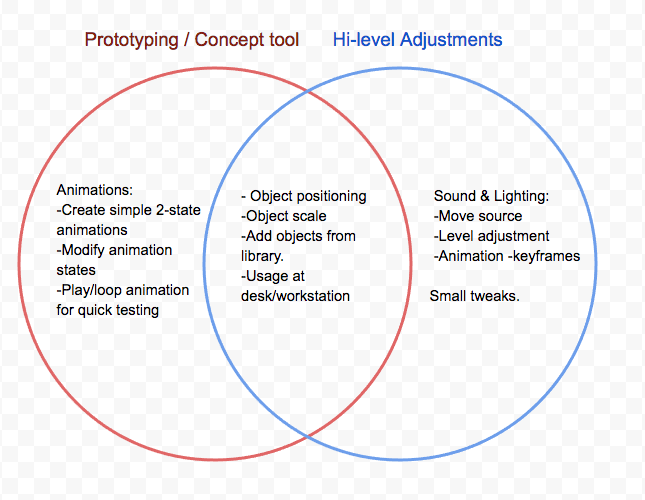
\includegraphics[width=.5\linewidth]{venn3.png}
  \caption{A diagram consisting of missing functionality when working with VR}
  \label{fig:result:interview:venn}
\end{figure}
